\section{Supervisionado} 

\begin{frame}
    \frametitle{Tipos de Aprendizado}
    \vspace{0.2cm}
     \textbf{Aprendizado Supervisionado x Não Supervisionado}
     \vspace{0.2cm}
     
     \begin{itemize}
         \item Supervisionado:
     \end{itemize}
         O modelo é treinado com dados rotulados, ou seja, dados em que já se sabe a resposta correta. (Regressão, Classificação).

    \vspace{0.3cm}
    
    \begin{itemize}
        \item Não Supervisionado:
     \end{itemize}
         O modelo encontra padrões ou grupos sem rótulos, ou seja, dados em que não se sabe a resposta correta. (Clustering/Agrupamento).
\end{frame}

\begin{frame}{Tipos de Aprendizado}
    \begin{center}
    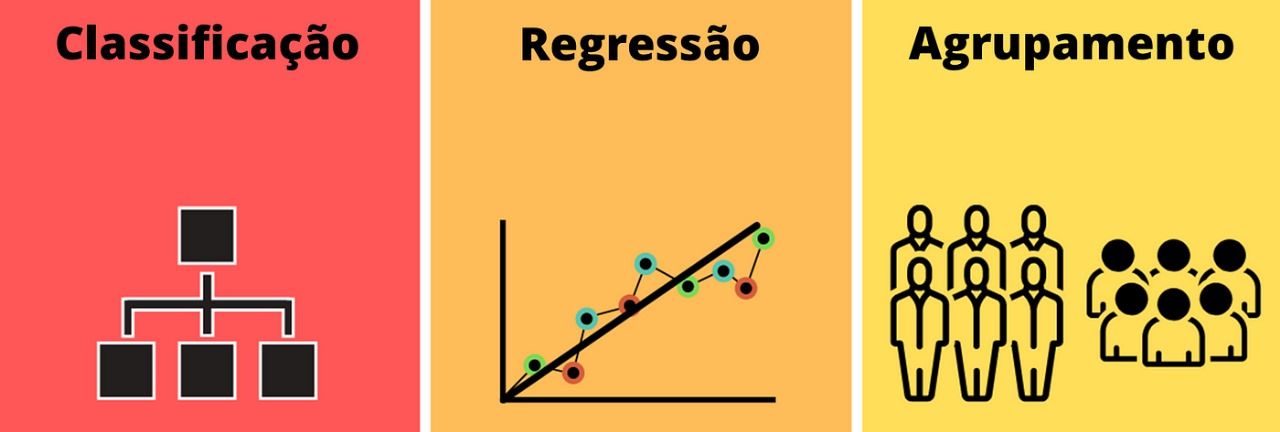
\includegraphics[width=1.0\linewidth]{img/TiposAprendizado.jpg}
    
    \end{center}
\end{frame}

\begin{frame}
    \frametitle{Aprendizado Supervisionado}
    \begin{figure}
        \centering
        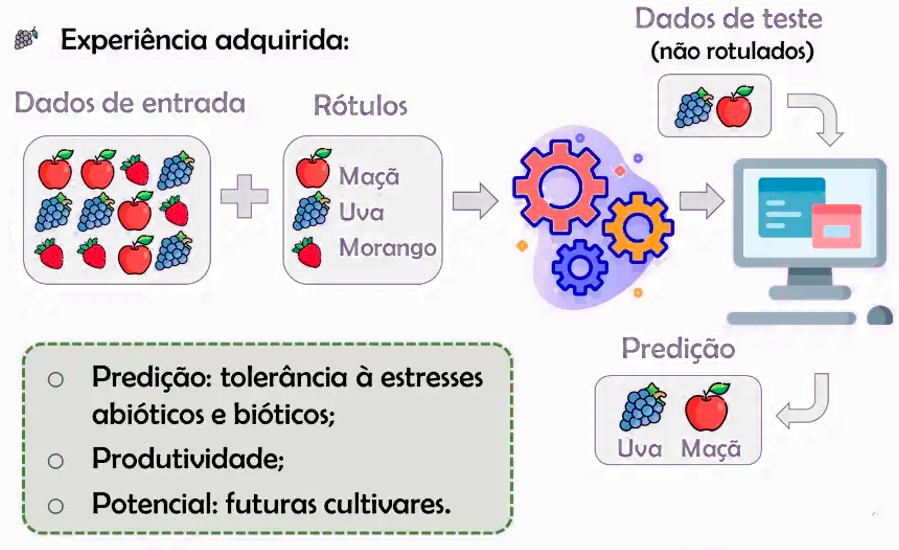
\includegraphics[width=1\linewidth]{img/supervisionado.png}
    \end{figure}
\end{frame}

\begin{frame}
    \frametitle{Classificação}
    \begin{itemize}
        \item Entender, reconhecer padrões e agrupar o conjunto de dados em categorias.
        \item Prever a categoria
    \end{itemize}
    \begin{figure}
        \centering
        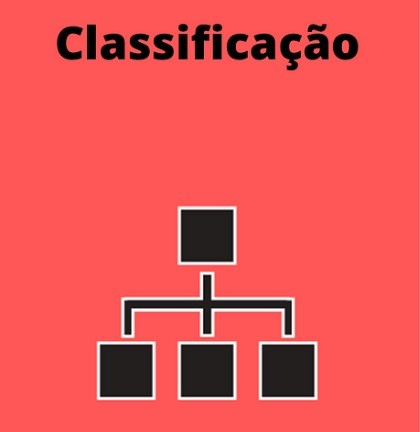
\includegraphics[width=0.3\linewidth]{img/Classificacao.jpg}
        \hspace{1cm}
        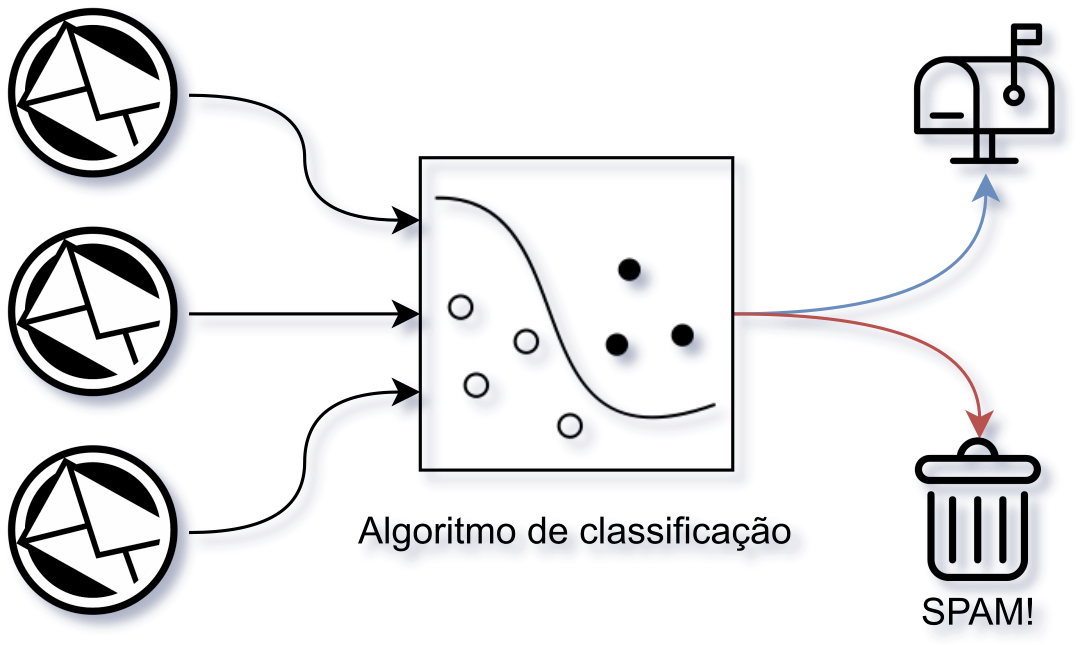
\includegraphics[width=0.5\linewidth]{img/ClassificacaoImagem.png}
    \end{figure}
\end{frame}

    \begin{frame}{Classificação}
    \textbf{Exemplos:}
    \begin{itemize}
        \item \textbf{Classificação de Gêneros Musicais:} Um modelo pode classificar uma música em múltiplos gêneros (ex.: rock e jazz).
        \item \textbf{Classificação de Rótulos de Produtos: }
        Atribuir um rótulo (como eletrônicos, vestuário, alimentos) a um produto com base em sua descrição.
        \item \textbf{Diagnóstico Médico: } Um classificador que utilize dados não observados de um paciente e classifique-o como doente ou não-doente.
    \end{itemize}
\end{frame}


\begin{frame}
    \frametitle{Matriz de Confusão}
    \begin{figure}
        \centering
        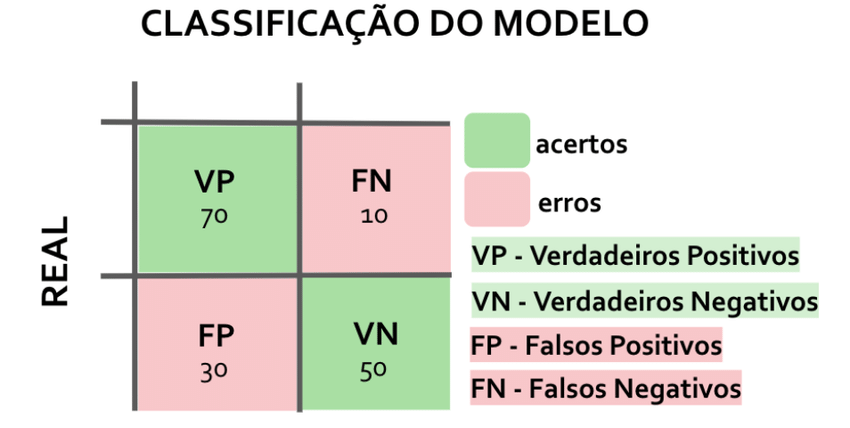
\includegraphics[width=0.8\linewidth]{img/MatrizConfusao.png}
    \end{figure}
    Usada para avaliar o desempenho de modelos de classificação.
\end{frame}

\begin{frame}
    \frametitle{Acurácia e Precisão}
    \textbf{Acurácia}
    \begin{itemize}
        \item Mede a proporção de \textbf{previsões corretas} (positivas e negativas) em relação ao total de previsões feitas.
    \end{itemize}

    \begin{center}
    \[
    Acuracia = \frac{VP + VN}{VP + VN + FP+ FN}
    \]
    \end{center}

    \textbf{Precisão}
    \begin{itemize}
        \item Mede a proporção de \textbf{previsões positivas} que estão realmente corretas.
        \item "Das vezes que o modelo previu positivo, quantas vezes ele estava certo?"
    \end{itemize}

    \begin{center}
    \[
    Precisao = \frac{VP}{VP + FP}
    \]
    \end{center}
    
\end{frame}

\begin{frame}
    \frametitle{Recall e F1 Score}
    \textbf{Recall}
    \begin{itemize}
        \item "Dos exemplos realmente positivos, quantos o modelo conseguiu prever corretamente?"
    \end{itemize}

    \begin{center}
    \[
    Recall = \frac{VP}{VP + FN}
    \]
    \end{center}

    \textbf{F1 Score}
    \begin{itemize}
        \item Média harmônica entre Precisão e Recall.
        \item Equilibra as duas métricas.
    \end{itemize}

    \begin{center}
    \[
    F1 Score = 2*\frac{Precisao*Recall}{Precisao + Recall}
    \]
    \end{center}
    
\end{frame}

\begin{frame}{Não devemos olhar só a acurácia!}
    \begin{figure}
        \centering
        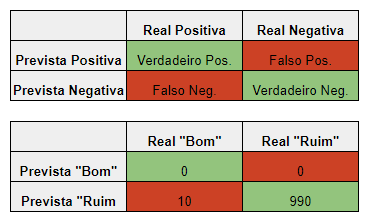
\includegraphics[width=0.5\linewidth]{img/MatrizComValores.png}
    \end{figure}
    \textbf{Dataset desbalanceado}
    \begin{itemize}
        \item 990 "Ruim"
        \item 10 "Bom"
    \end{itemize}

    \textbf{Modelo classifica tudo como "Ruim"}
    \begin{itemize}
        \item Acurácia: 99\%
        \item Recall: 0\%
    \end{itemize}
    
\end{frame}

\begin{frame}
    \frametitle{Regressão}
    \begin{itemize}
        \item Encontrar uma \textbf{função} que relacione as variáveis de entrada com a variável de saída.
    \end{itemize}
    \begin{figure}
        \centering
        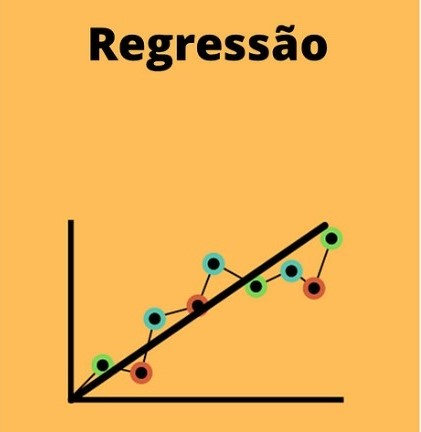
\includegraphics[width=0.3\linewidth]{img/Regressao.jpg}
        \hspace{0.2cm}
        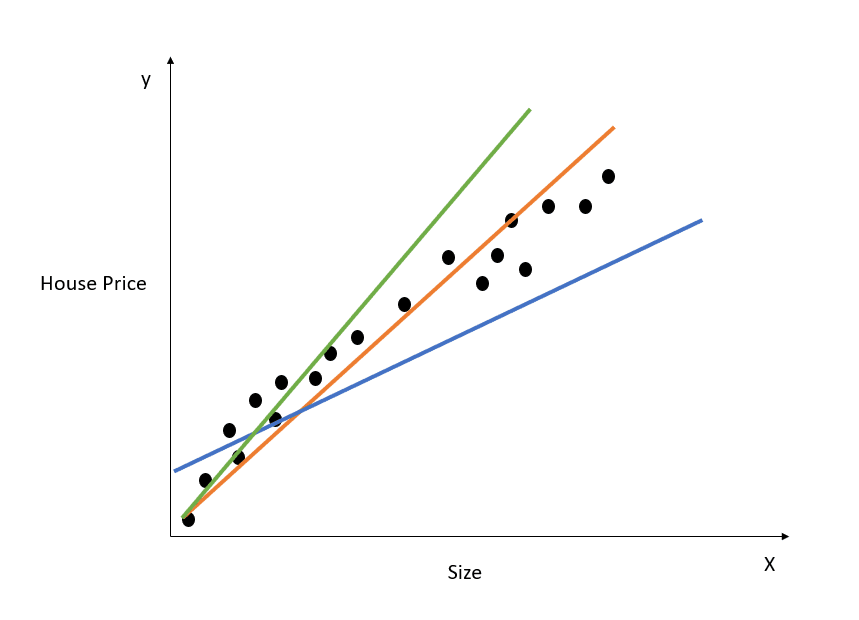
\includegraphics[width=0.5\linewidth]{img/RegressaoImagem.png}
    \end{figure}
    \begin{itemize}
        \item A linha \textbf{laranja} é a mais próxima de todos os pontos de dados mostrados.
        \item "Linha de Melhor Ajuste".
    \end{itemize}
\end{frame}

\begin{frame}
    \frametitle{Mean Absolut Error - MAE}
    \begin{itemize}
        \item Média da diferença entre o real e o previsto.
        \item valores maiores ou iguais a zero (módulo).
    \end{itemize}
    
   \begin{figure}
        \centering
        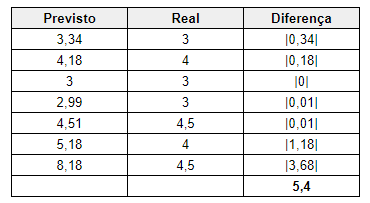
\includegraphics[width=0.6\linewidth]{img/TabelaMAE.png}
        \hspace{0.2cm}
        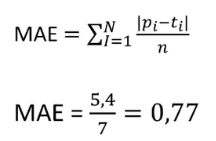
\includegraphics[width=0.3\linewidth]{img/MAEGabarito.png}
    \end{figure}
\end{frame}

\begin{frame}{Root Mean Squared Error - RMSE}
    \begin{itemize}
        \item Penaliza erros maiores de forma mais severa (quadrado).
        \item \textbf{Baixo RMSE:} O modelo está prevendo os valores reais com maior precisão.
        \item \textbf{Alto RMSE:} O modelo está cometendo erros significativos nas previsões.
    \end{itemize}
\end{frame}

\begin{frame}{Root Mean Squared Error - RMSE}

    \begin{figure}
        \centering
        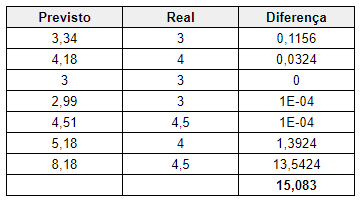
\includegraphics[width=0.6\linewidth]{img/TabelaRMSE.png}
        \hspace{0.2cm}
        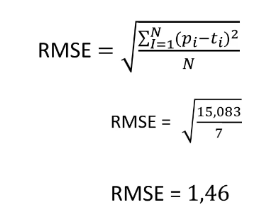
\includegraphics[width=0.4\linewidth]{img/RMSEGabarito.png}
    \end{figure}

\end{frame}

\begin{frame}{KNN}
    \begin{itemize}
        \item K-nearest neighbors, ou “K-vizinhos mais próximos”

        \item  Se os vizinhos mais próximos forem majoritariamente de uma classe, a amostra em questão será classificada nesta categoria.
        
    \end{itemize}
    \begin{figure}
        \centering
        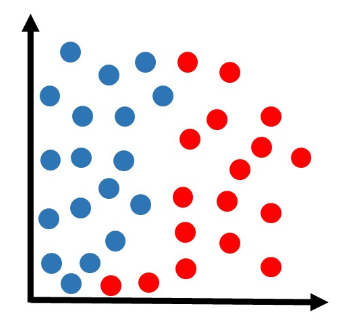
\includegraphics[width=0.20\linewidth]{img/KNN1.png}
    \end{figure}    
    
    \begin{figure}   
        \centering
        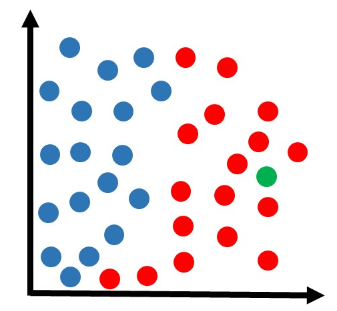
\includegraphics[width=0.20\linewidth]{img/KNN2.png}
        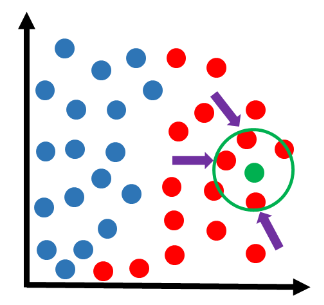
\includegraphics[width=0.20\linewidth]{img/KNN3.png}
        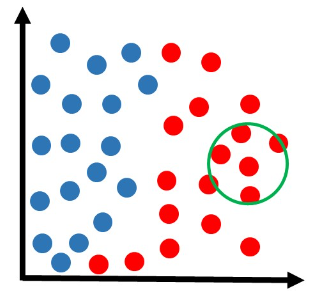
\includegraphics[width=0.20\linewidth]{img/KNN4.png}
    \end{figure}
\end{frame}

\begin{frame}
    \frametitle{Naive Bayes}
    \begin{itemize}
        \item Baseado no Teorema de Bayes de probabilidades condicionais.   
        \item Ideal para casos em que os dados podem se sobrepor entre si
    \end{itemize}

    \[P(C|X) = \frac{P(X|C) * P(C)}{P(X)}\]
    \centering
    \textit{\scriptsize{X: Data, C: Classe}} \\
    \scriptsize{"Qual a chance desse dado pertencer a categoria C dado que ele é um dado X?"}

    
    \begin{figure}
            \centering
            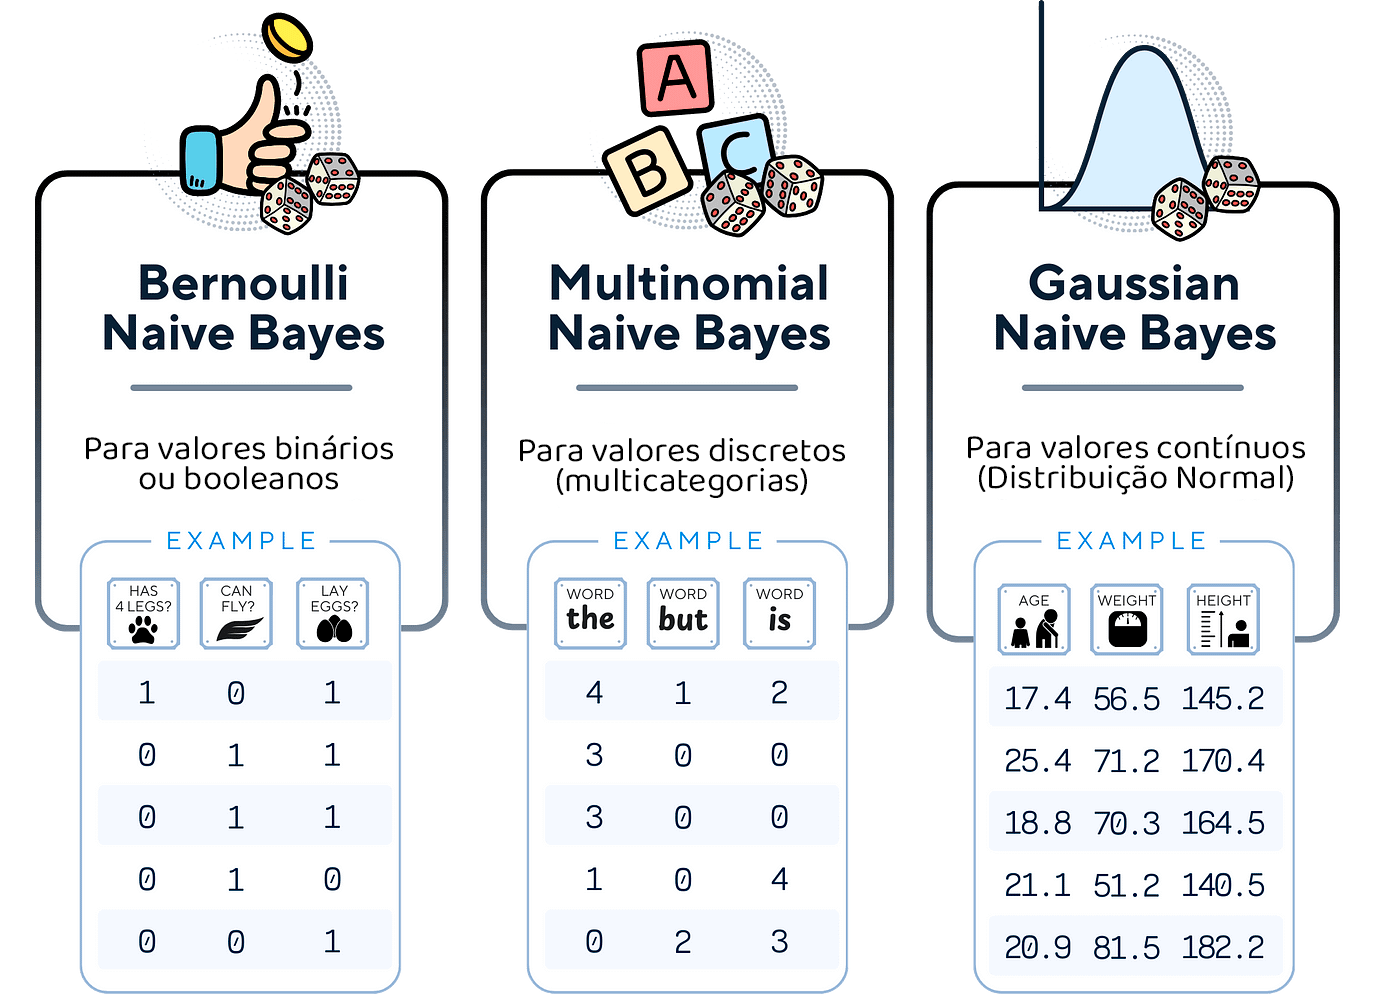
\includegraphics[width=0.5\linewidth]{img/naivebayes.png}
    \end{figure}
\end{frame}

\begin{frame}
    \frametitle{Árvore de Decisão (Decision Trees)}
    \begin{itemize}
        \item Vários pontos de decisão serão criados (nós).
        \item Em cada nó, o resultado da decisão será seguir por um caminho, ou por outro.
        \item  Uma pergunta será feita e teremos duas opções de resposta: sim ou não. A opção “sim” levará a uma próxima pergunta, e a opção “não” a outra.
    \end{itemize}
    \begin{figure}
        \centering
        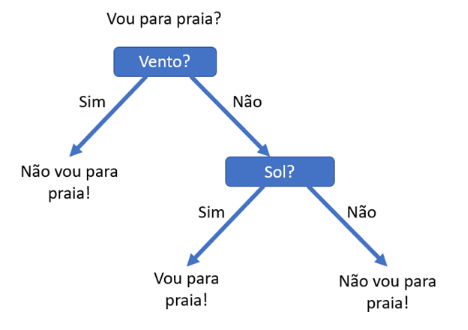
\includegraphics[width=0.5\linewidth]{img/ArvoreDecisao.png}
    \end{figure}
\end{frame}

\begin{frame}
    \frametitle{Floresta Aleatória (Random Florest)}
    \begin{itemize}
        \item Técnica de ensemble, ou seja, combina vários modelos para produzir um modelo final mais robusto.
        \item Constrói múltiplas Árvores de Decisão durante o treinamento e faz a média das previsões para melhorar a precisão e controlar o overfitting.
    \end{itemize}
    \begin{figure}
        \centering
        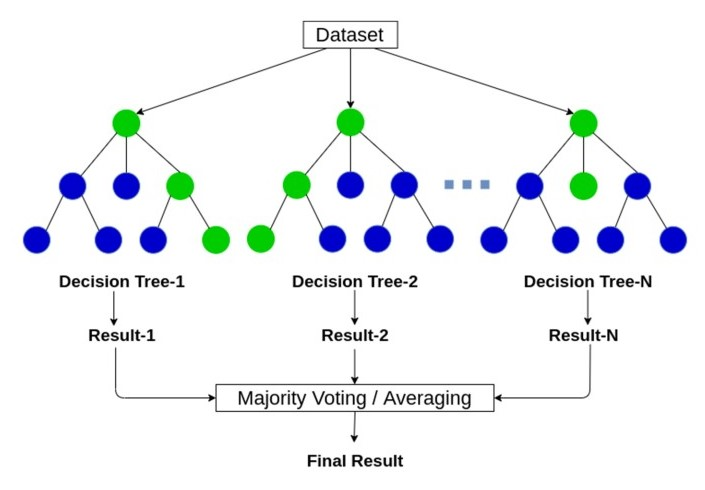
\includegraphics[width=0.5\linewidth]{img/randomflorest.jpeg}
    \end{figure}
\end{frame}
